\section{Design patterns: identification and analysis}
\label{sec:pattern_analysis}

\localtableofcontents
\newpage

The section at hand treats the question of introducing, and removing, design patterns in the context of an open source software project, in our case study, the MINA project. MINA has been analysed using the PACITO tool proposed in \cite{pacito}; PACITO has been extended and adapted to better fit our needs as described in section \ref{sec:pacito_dev}. The outcome of applying PACITO on the MINA code base is a dataset which comprises of historical data of design patterns instances which have appeared over the entire commit history of the MINA 2.1.X GitHub branch \cite{mina-github}. This branch corresponds with MINA version 2.1.3 analysed in this report.

Our approach to understanding the rationale behind introducing and removing patterns in MINA is to analyse the issue from two perspectives: on one hand, we conduct a quantitative analysis based on the extracted dataset combined with our knowledge of the system and its complexity, on the other hand, we select individual pattern instances from the dataset and cross reference the obtained information from PACITO with other sources (i.e. mailing list, JIRA issues, previous system architectures) in order to gather concrete insight into the decision of introducing or removing patterns. Finally, we combine the results of these two approaches and we conclude by answering the following research questions:
\begin{enumerate}
    \item Why are design patterns introduced? Are design patterns implicitly or explicitly introduced?
    \item Why are design patterns removed?
    \item Are design patterns related decisions discussed among developers?
\end{enumerate}

\subsection{Recovered patterns dataset pre-processing}
Prior to analysing the dataset, certain pre-processing steps were required. We observed that sometimes PACITO recovers the same pattern multiple times for a specific class: for example it will find a new Adapter instance for every method that is being adapted, or it will find a new Factory instance for every method on the same Factory class. We decided to merge these occurrences in what we will refer to for the rest of the section as a \textit{pattern instance}. A \textit{pattern instance} is defined by a recovered pattern, a class file (i.e. corresponding to the implementation) and its implementation which can consist of multiple properties.

A \textit{pattern instance} is also bounded by an \textit{introCommit} and \textit{outroCommit}. To better exemplify this, if the implementation of a pattern in a certain class changes (e.g. some properties change), a new \textit{pattern instance} will be introduced, while the previous one will be regarded as removed since the code base does not reflect its implementation any longer.

Another aspect we observed was related to commit \#1851; this commit captures a module refactoring, pattern instances being reintroduced in the same scopes, however, with different names.
We cross-matched the recovered patterns before this commit (in accordance to the definition of a \textit{pattern instance}, therefore we also took into consideration the implementation, not only the class file names) with the renamed pattern instances; for consistency, we merge the correlated \textit{pattern instances}.\\\\
Before these pre-processing step the dataset contained a total of 2586 recovered patterns, while after the pre-processing, the number dropped to 1882 pattern instances.

\subsection{Quantitative analysis: recovered patterns dataset analysis}
The recovered patterns dataset includes 1882 data points which represent pattern instances in the MINA code base. Out of the 1882 instances, 1802 have been removed from the project, currently, 80 pattern instances still being included in the stable code base of version 2.1.3. These numbers are not surprising since the entire commit history has been analysed (approx. 2546 commits out of which 551 commits were relevant to the topic of this analysis), however \textbf{the number of currently included pattern instances is relatively high, considering the open source nature of the project and that no clear architecture has been initially defined} (few mentions about architectural decisions regarding the usage of design patterns in the documentation). Moreover, the significant number of pattern instances removals (almost as large as the number of commits) indicate \textbf{a fast pace of architectural and implementation changes throughout the development phase.} This might lead to a preliminary conclusion that \textbf{design patterns are introduced out of necessity for solving complex problems and they arise from the experience of the developers, rather than being the blueprint of the software to be developed.}

\subsubsection{Overview of recovered patterns \& rate of pattern changes}
Figures \ref{fig:pattern_occ_all} presents an overview of the occurrence of pattern instances overall, while figures \ref{fig:pattern_occ_current} and \ref{fig:pattern_occ_removed} in Appendix \ref{sec:quantitative_analysis_figures}, present the pattern occurrences in the current code version of the MINA 2.1.3 project and, respectively, the removed pattern instances. 

\begin{figure}
    \centering
    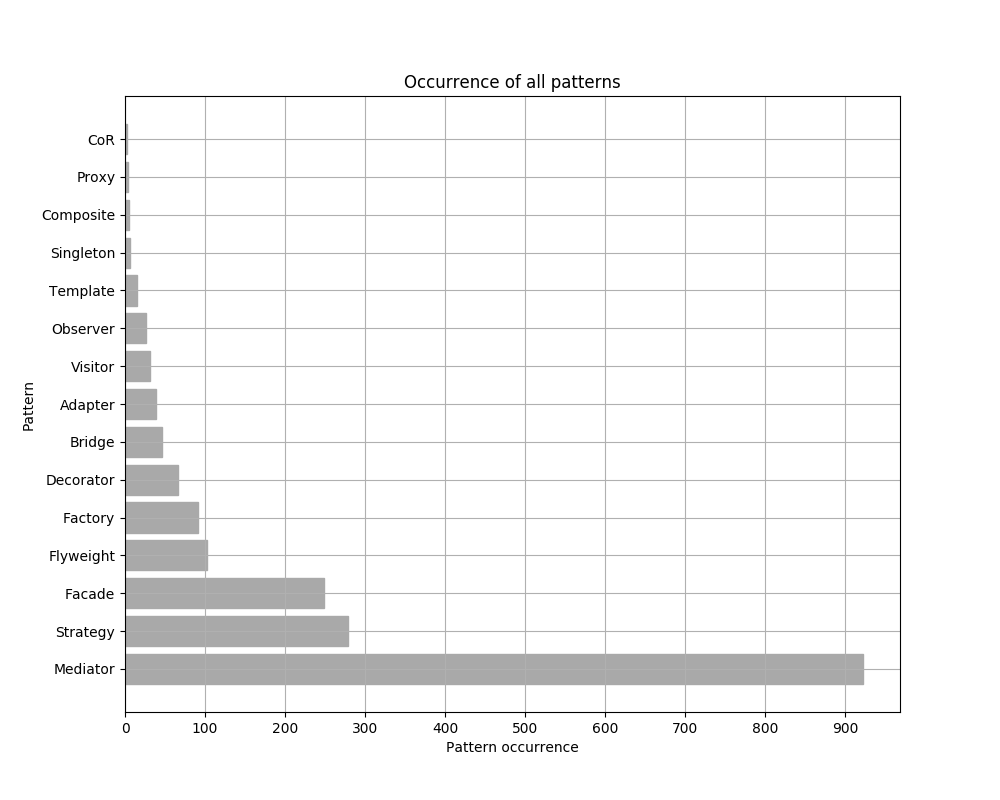
\includegraphics[width =  \textwidth]{images/graphs/pattern_occurrence_all.png}
    \caption{Overview of all pattern instances retrieved from the entire commit history of MINA 2.1.3. 15 different patterns have been introduced, with the \texttt{Mediator} and \texttt{Strategy} pattern having the most occurrences.}
    \label{fig:pattern_occ_all}
\end{figure}

Overall, 15 different patterns have been recovered, currently, 11 out of the 15 are present. Following the GoF (Gang of Four) \cite{gof} design pattern classification, most patterns used are either structural (e.g. Decorator, Facade, Adapter, Bridge, Flyweight) or behavioural (e.g. Strategy, Mediator, Observer, Chain of Responsibility, Template, Visitor). \textbf{The most used patterns are, by far, the Strategy and Mediator patterns.} The Strategy pattern allows the choice of an algorithm at run time from a family of previously defined algorithms. In the context of MINA, this pattern could be suitable in multiple instances, for example for the transport, filtering and handler components. The Mediator pattern allows loose coupling between classes by enabling interaction that do not require the participating classes to have any knowledge of each other. This pattern achieves high modifiability through encapsulation and could have been applied anywhere in the scope of the MINA project. \textbf{The striking large number of occurrences of these two patterns (especially for the Mediator pattern which is recovered more than 900 times over the entire project) is tackled by an equally large number of removals (i.e. approx. 900 removals for the Mediator pattern, see figure \ref{fig:pattern_occ_removed}) in Appendix \ref{sec:quantitative_analysis_figures}} which shows the superfluous nature of introducing patterns in cases that do not fit the pattern context. \textbf{This also points to a tendency towards redundancy in the development of MINA.}
\begin{figure}[H]
    \centering
    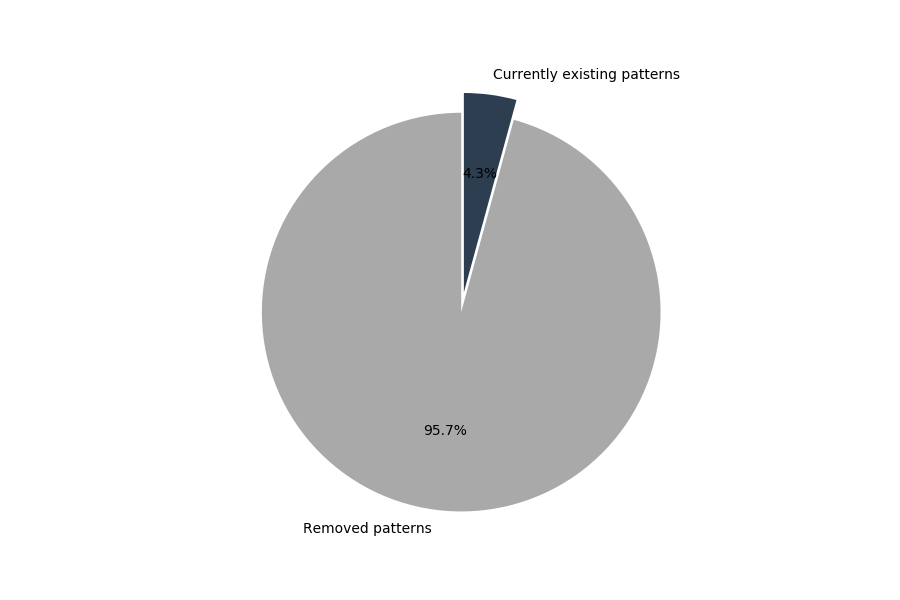
\includegraphics[width =  \textwidth]{images/graphs/current_removed_per.png}
    \caption{Percentage of removed pattern instances out of all recovered patterns.}
    \label{fig:per_removed_patterns}
\end{figure}
The variation between introducing and removing patterns is also captured by figure \ref{fig:per_removed_patterns}. Out of the total number of pattern instances recovered with PACITO, 95.7\% of them have been removed. This re-enforces our previous statement that \textbf{the patterns in discussion have been introduced after establishing the initial architecture, following rather a trial and error strategy, rather than a pattern driven model for architecture modelling} (for example, the proposed PDAP methodology proposed in \cite{pdap}). Even though design patterns offer proven solutions to complex, reoccurring problems, they inherently require more attention to implementation and imply certain trade-offs or implications. These implications of introducing patterns \textit{a posteriori} might have led to the high variation between additions and removals, for example issues such as increased code complexity, cross cutting concerns, increased development and maintenance time might have been potential reasons for pattern removals.

\begin{figure}[H]
    \centering
    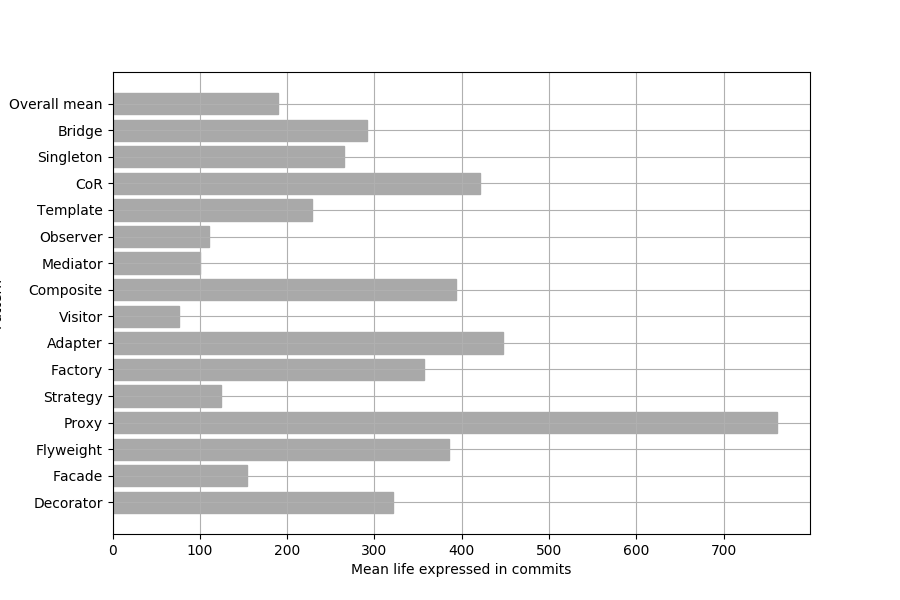
\includegraphics[width =  \textwidth]{images/graphs/mean_life.png}
    \caption{Median lifespan expressed in commits for the removed patterns.}
    \label{fig:mean_life}
\end{figure}

The mean lifespan, expressed in number of commits, of the identified patterns is presented in figure \ref{fig:mean_life}. From the figure, it is apparent that the mean lifespan of the Proxy pattern instances is an outlier. For this graph, we must consider that PACITO  accounts for `gaps' between removal and a new addition of the same pattern instance, which results into significantly large values. The existence of `gaps' offers insights into the inconsistencies in development: a decision to add, remove and then add again a pattern instance for the same scope of the project is proof of the fragmented thought process of the development community. However, this is not out of the ordinary for an open software project which implies a volatile development team structure and lack of centralized decision making. \textbf{The median `life expectancy' of a pattern instance is of approx. 50 commits, which is approx. 9\% out of the total number of commits made. This can be translated into a high velocity of structural changes.}

\subsubsection{Rate of pattern introductions and removals at commit level}
The commit history analysed can be classified into 3 categories: commits which introduce new pattern instances (i.e. intro commits), commits which remove existing pattern instances (i.e. outro commits) and the combination of the two (i.e. intro/outro commits). The distribution of the 3 commit types over the entire extracted dataset is presented in figure \ref{fig:pattern_commit_percentage}. 
\begin{figure}[H]
    \centering
    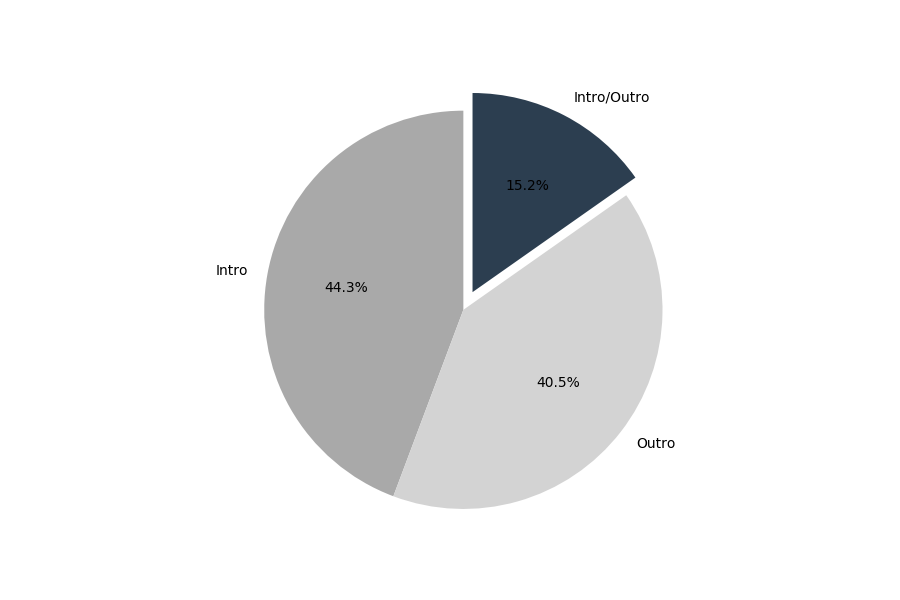
\includegraphics[width =0.9\textwidth]{images/graphs/intro_outro_per.png}
    \caption{Distribution of pattern instances introductions and removals over the analysed commits.}
    \label{fig:pattern_commit_percentage}
\end{figure}

The percentage of intro and outro commits are approx. equal (i.e. 44.3\% and 40.5\%, respectively); \textbf{this can be regarded as an indicator that most of the pattern instances introduced have been invariably removed after a period of time (see figure \ref{fig:mean_life}).} Keeping in mind the large number of pattern instances recovered (i.e. 1882 pattern instances), we reach our second preliminary conclusion that, \textbf{in the context of MINA, a quantitative rather than a qualitative approach has been taken w.r.t. the patterns used} (one might argue that this volatility could have been influenced by changes in requirements, however, we will show in section \ref{sec:scope_analysis} that the scopes of most of the patterns overlap with the \texttt{core} component of MINA which has been stable in terms of features/functional requirements since its initial version).  

The intro/outro commits imply additional complexity: a pattern instance removal is followed by the introduction of a more suitable pattern, for example. Figure \ref{fig:add_rem_commit} shows an account of pattern introductions and removals per commit. The visualisation capture the workflow of the development team which corresponds to small and more frequent commits.

\begin{figure}[H]
    \centering
    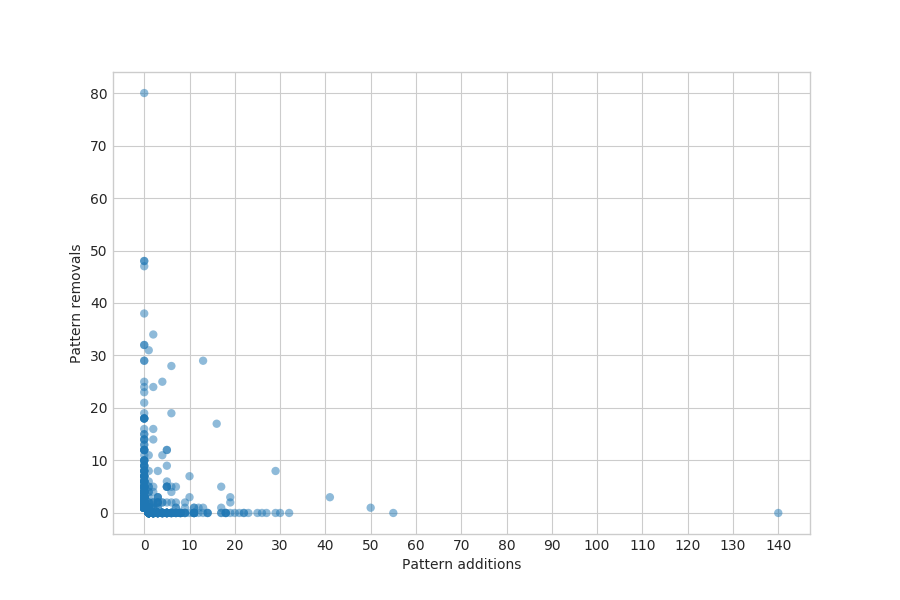
\includegraphics[width = 0.9\textwidth]{images/graphs/additions_removals_commit.png}
    \caption{Pattern instances additions and removals per commit.}
    \label{fig:add_rem_commit}
\end{figure}

 As predicted from the previous figure (see figure \ref{fig:pattern_commit_percentage}), the (0, y) axis (corresponding to outro commits) is similar to the (x, 0) axis (corresponding to intro commits), the most evident difference is that intro commits are spread in the [0, 30] interval (more focused in the [0, 15] interval) and can span up until over 30 additions per commit (commits exceeding this bound are considered outliers). The outro commits also span the [0, 30] interval, but increase consistently. \textbf{Pattern removals are therefore more consistent and iterative, while additions are generally kept towards the lower bound, but can appear sporadically and have a greater impact by introducing a large number of pattern instances at once.} The intro/outro commits are bounded by the 15 additions/removals limit. Given this bound, their impact is comparatively less significant, therefore they might be intended for improvements or switching patterns for more suitable alternatives, while still preserving the global pattern occurrences. 



Figure \ref{fig:commit_timeline} presents a timeline of the evolution of the total number of patterns in the code base in accordance with the analysed commits. \textbf{The pattern data shows as descending trend}; the peak was reached around commit \#300 (roughly capturing the start of the development phase of MINA version 1.0.0), reaching a plateau-like state around commits \#1500 - \#2300; most recently, following a decrease below 100 patterns. \textbf{This decrease shows a tendency towards stabilization, which follows from the fact that the project is reaching towards its maturity (already version 2.1.3).} The phase when much of the volatility and changes in terms of patterns seem to have occurred is the period between commit \#600 and \#1200 - \#1500 (which roughly correspond to the development of versions 2.0.X).  

\begin{figure}[H]
    \centering
    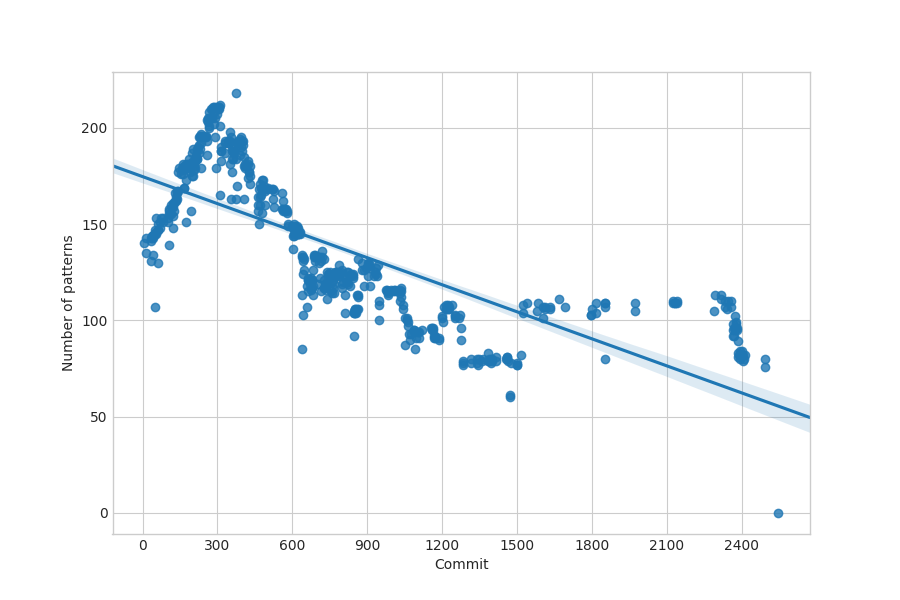
\includegraphics[width =0.9\textwidth]{images/graphs/commit_timeline.png}
    \caption{Timeline of analysed commits as expressed by the total number of pattern occurrences at the time of the commit. The timeline is fitted with a linear regression.}
    \label{fig:commit_timeline}
\end{figure}

\subsubsection{Distribution of patterns over the MINA components scope}
\label{sec:scope_analysis}
Design patterns are usually introduced for the main purpose of facilitating the implementation of a proven to a complex, reoccurring problem. This leads to the investigation of the scope of the introduced patterns: by understanding \textit{where} they have been introduced, one might be able to infer the \textit{why}. Figure \ref{fig:scope_percentages} shows the distribution of all the patterns recovered in accordance to their implementation scope within the MINA code base (names might differ since the entire commit history has been considered). Figure \ref{fig:others_scope_percentages} in Appendix \ref{sec:quantitative_analysis_figures} complements figure \ref{fig:scope_percentages}. \textbf{The most prominent component is the \texttt{core}}; as described in section \ref{sec:analysis_components}, it is the backbone of MINA and offers the basic functionalities required to implement a MINA based application. \textbf{Having the most patterns concentrated over this component is not surprising, since it is also the most extensive component.}

Other components that entail a significant complexity are the ones implementing the \texttt{http} support (patterns such as Proxy, Strategy could be considered here)  and the \texttt{integration} modules (patterns such as Facade would be suitable in this case). The \texttt{mina-statemachine} component also entails a high level of complexity since it aims at implementing an improved version of the State pattern.

\begin{figure}[H]
    \centering
    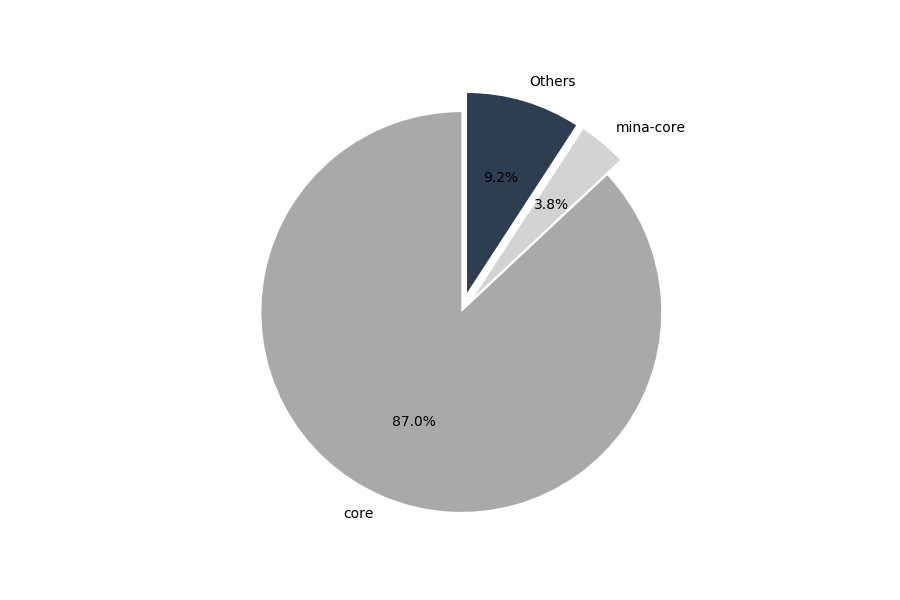
\includegraphics[width =\textwidth]{images/graphs/all_scopes_per.png}
    \caption{Code base component scopes of the recovered patterns from the entire commit history.}
    \label{fig:scope_percentages}
\end{figure}

The pattern distribution in the current code base version of MINA is reflected in figure \ref{fig:current_scopes_percentages}. The information depicted in this figure follows the overall pattern distribution presented in the figures above (figures \ref{fig:scope_percentages} and \ref{fig:others_scope_percentages} in Appendix \ref{sec:quantitative_analysis_figures}). Some changes are apparent: for instance, there is no recovered pattern spanning the \texttt{http} related components any more. This might be an indication of the fact that the actual implementation has strayed from the expected pattern implementation, even though the concept is still followed. This might come as a consequence to the fact that design patterns require a certain level of knowledge and understanding in order to achieve a successful implementation. Also, some integration components (i.e. \texttt{jmx}, \texttt{spring}) are no longer supported by patterns (their complexity might have been overestimated).
\begin{figure}
    \centering
    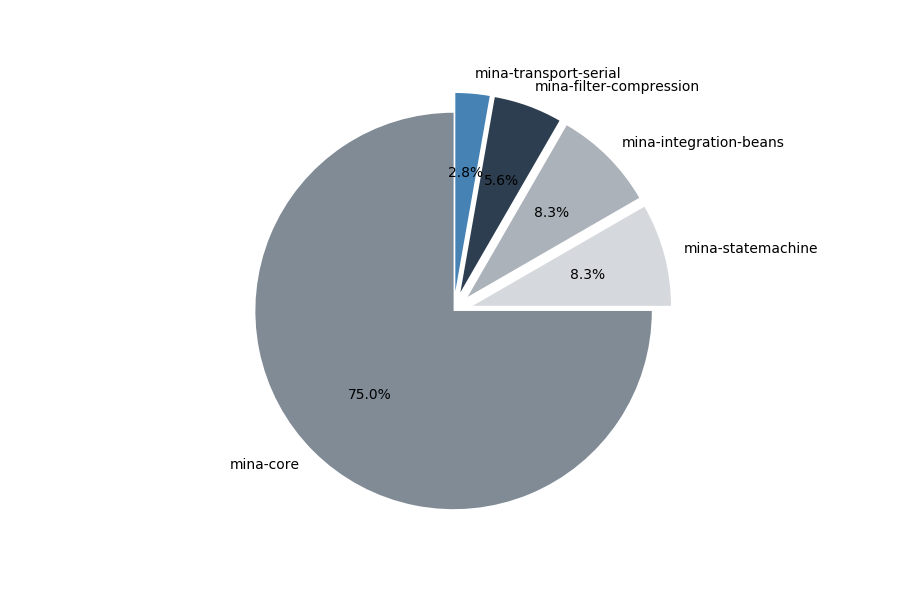
\includegraphics[width =0.9\textwidth]{images/graphs/current_scopes_per.png}
    \caption{Distribution of current pattern instances over all the components of the MINA project. \texttt{mina-core} includes the \texttt{core} component.}
    \label{fig:current_scopes_percentages}
\end{figure}

Figure \ref{fig:mina_core_scope}, in Appendix \ref{sec:quantitative_analysis_figures}, narrows the scope to more specific areas of the code base where current patterns exist. From this diagram, the intricacy of the component implementation becomes clear: the most occurrences appear over components that support the implementation of the \texttt{filter} components; following the component descriptions in section \ref{sec:analysis_components}, through the \texttt{filtering} components,  additional functionality of processing networking communication is provided. Since various filters of different complexities are provided out-of-the-box, it follows logically that the filtering components would require more attention to tackle the various complexities entailed. Components that support the networking \texttt{transport}, as well as the \texttt{service} and \texttt{session} components, are also spanned by multiple pattern occurrences; these are complex components that bind together all necessary elements for establishing the baseline connection between client and server, which resides at the backbone of any networking application. The \texttt{byteaccess} component contains the most pattern occurrences, respectively 8 pattern instances; this follows from the fact that basic data buffers are implemented from scratch in MINA.

\subsection{Qualitative analysis: individual patterns analysis}
\label{sec:qualitative_analysis}
Following the quantitative analysis, we investigate a sample of recovered pattern instances individually. The sample includes both patterns that have been removed, as well as patterns that are currently implemented in the code base. The key aspects relevant to this investigation are the implementation of the patterns \footnote{We judge the Java implementation starting from the pattern definition for which we use online sources that are available to any developer; we assume that no academic understanding of design patterns is required}, as well as the motivation behind their introduction, and possible removal. The impact on the overall architecture (as presented in section \ref{sec:analysis_components}) is also considered.

\subsubsection{Current patterns: Facade \& Adapter patterns}
\label{sec:current_facade_adapter}
The implementation of the out-of-the-box prefixed codec filter uses both the Facade and Adapter patterns, as recovered by PINOT. We present and analyse these patterns as a whole as follows:

\textsc{Pattern definition}: 
\begin{itemize}
    \item \textsc{Facade} is a structural pattern which hides the complexities of a system by providing a simplified interface to said system. Implementation wise, Facade implies a single class or point-of-entry to the system which communicates with the user (or client) and provides simplified methods by delegating to underlying classes that are not directly visible to the user \cite{facade}\cite{facade1}.
    \item \textsc{Adapter} combines the functionalities of independent interfaces; it is also considered a structural pattern since it provides a means of communication between separate structural entities. It entails an adapter and adaptees: the adapter wraps the functionality of the adaptees in order to facilitate the service usage of the adaptees by an independent, incompatible client entity \cite{adapter}\cite{adapter1}.
\end{itemize}

\textsc{Pattern implementation information from PINOT}: 
\begin{itemize}
    \item PINOT has identified 2 Facade pattern instances which are complementary to one another with intro commit \#1205; we present them together:
        \begin{itemize}
            \item \textsc{Access point}: \texttt{PrefixedStringCodecFactory}
            \item \textsc{Facade}: \texttt{PrefixedStringEncoder}, \texttt{PrefixedStringDecoder}
            \item \textsc{Hidden complexity}: \texttt{IOBuffer}, \texttt{ProtocolEncoderOutput}, \texttt{ProtocolDecoderOutput}
            \item \textsc{Scope}: \texttt{mina-core/filter/codec/prefixedstring/}
        \end{itemize}
    \item The Adapter pattern has been recovered (at intro commit \#1851) for two adaptees (which coincide with the facades mentioned above) and one adapter:
        \begin{itemize}
            \item \textsc{Adapter class}: \texttt{PrefixedStringCodecFactory}
            \item \textsc{Adaptees}: \texttt{PrefixedStringEncoder}, \texttt{PrefixedStringDecoder}
            \item \textsc{Adapting}: \texttt{ProtocolCodecFactory}
        \end{itemize}
\end{itemize}

\textsc{Implementation \& class diagram}: The implementation is capture by figure \ref{fig:cd_facade}; the hidden complexity, as captured by PINOT, consists of the results of the prefixed encoding and decoding, as well as the \texttt{IOBuffer} which `stores' this data. These complexities are wrapped by the corresponding classes (i.e. \texttt{PrefixedStringEncoder} and \texttt{PrefixedStringDecoder}) which encapsulates them in the \texttt{encode} and, respectively, \texttt{doDecode} methods. These 2 classes cannot be directly accessed; they are created by the \texttt{PrefixedStringCodecFactory} which acts as the entry point: a user would interact with this class in order to use the functionality provided by the prefix codec. However, the \texttt{PrefixedStringCodecFactory} does not provide the additional layer of abstraction of delegating responsibilities to its underlying components: this implies that the user needs to be aware of the \texttt{encode} method of the \texttt{encoder} field of the \texttt{PrefixedStringCodecFactory} class in order to access the prefix encoding functionality. This also holds for the decoding step.

At the same time, the \texttt{PrefixedStringCodecFactory} is identified to be the adapter class which entails that it bridges incompatible interfaces; this recovery is an \textbf{incorrect detection} of the Adapter pattern. We motivate this statement as follows: the adaptees are identified as the \texttt{PrefixedStringEncoder} and \texttt{PrefixedStringDecoder} (they represent implementations of the \texttt{ProtocolEncoder} and \texttt{ProtocolDecoder} interfaces), therefore the \texttt{PrefixedStringCodecFactory} wraps these two classes in order to make them compatible to the adapting interface, \texttt{ProtocolCodecFactory}. However, the \texttt{PrefixedStringCodecFactory} implements \texttt{ProtocolCodecFactory} which, at the same time, has dependencies to the \texttt{ProtocolEncoder} and \texttt{ProtocolDecoder} interfaces. We, however, consider that the \texttt{PrefixedStringCodecFactory} is an instance of the Factory design pattern (as suggested by the name of the class) \cite{factory}: the \texttt{PrefixedStringCodecFactory} creates instances of the \texttt{PrefixedStringEncoder} and \texttt{PrefixedStringDecoder} interfaces.

\textsc{Issue tracking \& motivation}: The motivation for the patterns addition is the implementation of a fixed-length prefix encoding/decoding mechanism, where no additional information of delimiters between encoded values is necessary:

\textit{"added a codec for Java String objects using a fixed-length length prefix (and no delimiter)"}, commit message for intro commit \#1205 of the Facade pattern.

Moreover, the prefixed codec should be accessible as an out-of-the-box filter for the users developing their MINA based applications. We have identified 18 mentions in the official developer mailing list \cite{mina-mail} regarding the prefix codec which generally discuss the implementation of the codec, however, there is no direct mention of the Facade pattern in relation to this implementation (the keyword `facade' has been found 43 times, however, it broadly refers to the design pattern and it is found in relation with the logging SLF4J \cite{slf4j} functionality of MINA). As for the adapter pattern (identified by keyword `adapter'), there is no mention of it w.r.t. the prefixed codec, however, we have identified an extensive discussion within the developers' mailing thread regarding the confusing naming of files (file names contain the `adapter' keyword) in the absence of the adapter pattern named in the file name. Excerpts from the mailing lists show that the understanding (and/or discussion about the implementation) of the real pattern is limited:

\textit{"The *Adapter classes are convenience wrappers meant to be extended by the user if he only wants to use a "subset" of the interfaces they implement."}

\textit{"Again, these classes are \_not\_ adapters, w.r.t. the definition of the 
adapter pattern."}

\textsc{Impact on architecture}: The impact of the Facade and Adapter patterns on the structure of the overall architecture is not too significant since the scope of the patterns is rather self-contained and does not go beyond the \texttt{mina-core-filter} component. The same approach of using this combination of patterns is also identified for other types of filters within the same component, for example \texttt{ObjectSerializationCodecFactory} and \texttt{TextLineCodecFactory}, which also represent out-of-the-box implementations for processing communicated data.\\\\
\textsc{Preliminary conclusions}: The recovered instance analysed above can be considered a loose implementation of the Facade pattern, where the main goal seems to have been abstraction of complexity, with less focus on how to delegate this complexity such that the user is only coupled with a very simple system entry point. The lack of mentions and discussion about this topic points out to the possibility that the Facade pattern instance, in this specific case, might not have been intentional, but logically followed from respecting good object oriented Java practices, also considering that the Facade pattern does not entail a lot of complexity in itself. As for the Adapter pattern, the two interfaces that are being bridged (as recovered by Pinto) are connected through a dependency, therefore we cannot state that they are completely incompatible. The main motivation behind the adapter, in this particular case, was to expose and provide compatibility for the out-of-the-box codec implementation to the users and their MINA based applications, however this does not yield a correct implementation of this pattern, especially considering the pattern components identified by PINOT. \textbf{In this case, we can state that PINOT has incorrectly detected the Adapter pattern}. Instead, the adapter class can be seen as a good example of a Factory pattern instance.\\\\
\textsc{Similar pattern instances}:  Similar instances of the combination of Facade and Adapter patterns have been recovered within the \texttt{mina-core/filter/codec} scope for the \texttt{TextLineCodec} and \texttt{ObjectSerializationCodec}; the same pattern structured is followed as for the \texttt{PrefixedStringCodec} meaning that, in the context of the Facade pattern, \texttt{CodecNameFactory} class is the access point, while \texttt{CodecNameEncoder} and \texttt{CodecNameDecoder} classes are the facades. The Adapter pattern is again incorrectly detected for the \texttt{CodecNameFactory} classes. Given the similarities in structure, we are more interested in the motivation of introducing this combination of patterns for this 2 cases:
\begin{itemize}
    \item \texttt{TextLineCodec}
        \begin{itemize}
            \item \textsc{Intro commit numbers}: \#813, \#819 (Facade), \#1851 (Adapter)
            \item \textsc{Commit messages}: From the commit messages, we identify that the \texttt{TextLineEncoder} facade has been updated according to a refactoring which is traced by a JIRA issue (i.e. \textit{"DIRMINA-451 Rename org.apache.mina.common.ByteBuffer to IoBuffer to avoid confusion with NIO ByteBuffer"}). The \texttt{TextLineEncoder} facade has been introduce following a issue fix also traced to a JIRA issue (i.e. \textit{"Related issue: DIRMINA-454 (Trivial denial of service in TextLineDecoder)"}). The Adapter pattern has been recovered at commit \#1851 which marks the module refactoring.
            \item \textsc{Developer discussion}: no discussion about patterns related to the implementation of the \texttt{TextLineCodec}.
        \end{itemize}
    \item \texttt{ObjectSerializationCodec}:
    \begin{itemize}
        \item \textsc{Intro commit numbers}: \#813 (Facades), \#1851 (Adapter)
        \item \textsc{Commit messages}: The \texttt{ObjectSerializationEncoder} and \texttt{ObjectSerializationDecoder} facades have been recovered in relation to a intro commit that marks a refactoring (i.e. \textit{"DIRMINA-451 Rename org.apache.mina.common.ByteBuffer to IoBuffer to avoid confusion with NIO ByteBuffer"}). The Adapter pattern has been recovered at commit \#1851 which marks the module refactoring.
        \item \textsc{Developer discussion}: no discussion about patterns related to the implementation of the \texttt{ObjectSerializationCodec}.
    \end{itemize}
\end{itemize}
\textsc{Total number of pattern instances analysed:} 10 pattern instances:
\begin{itemize}
    \item \textsc{Facade pattern}: 7 pattern instances corresponding to intro commits \#813, \#819, \#1205.
    \item \textsc{Adapter pattern}: 3 pattern instance corresponding to intro commit \#1851.
\end{itemize}

\begin{figure}[H]
    \centering
    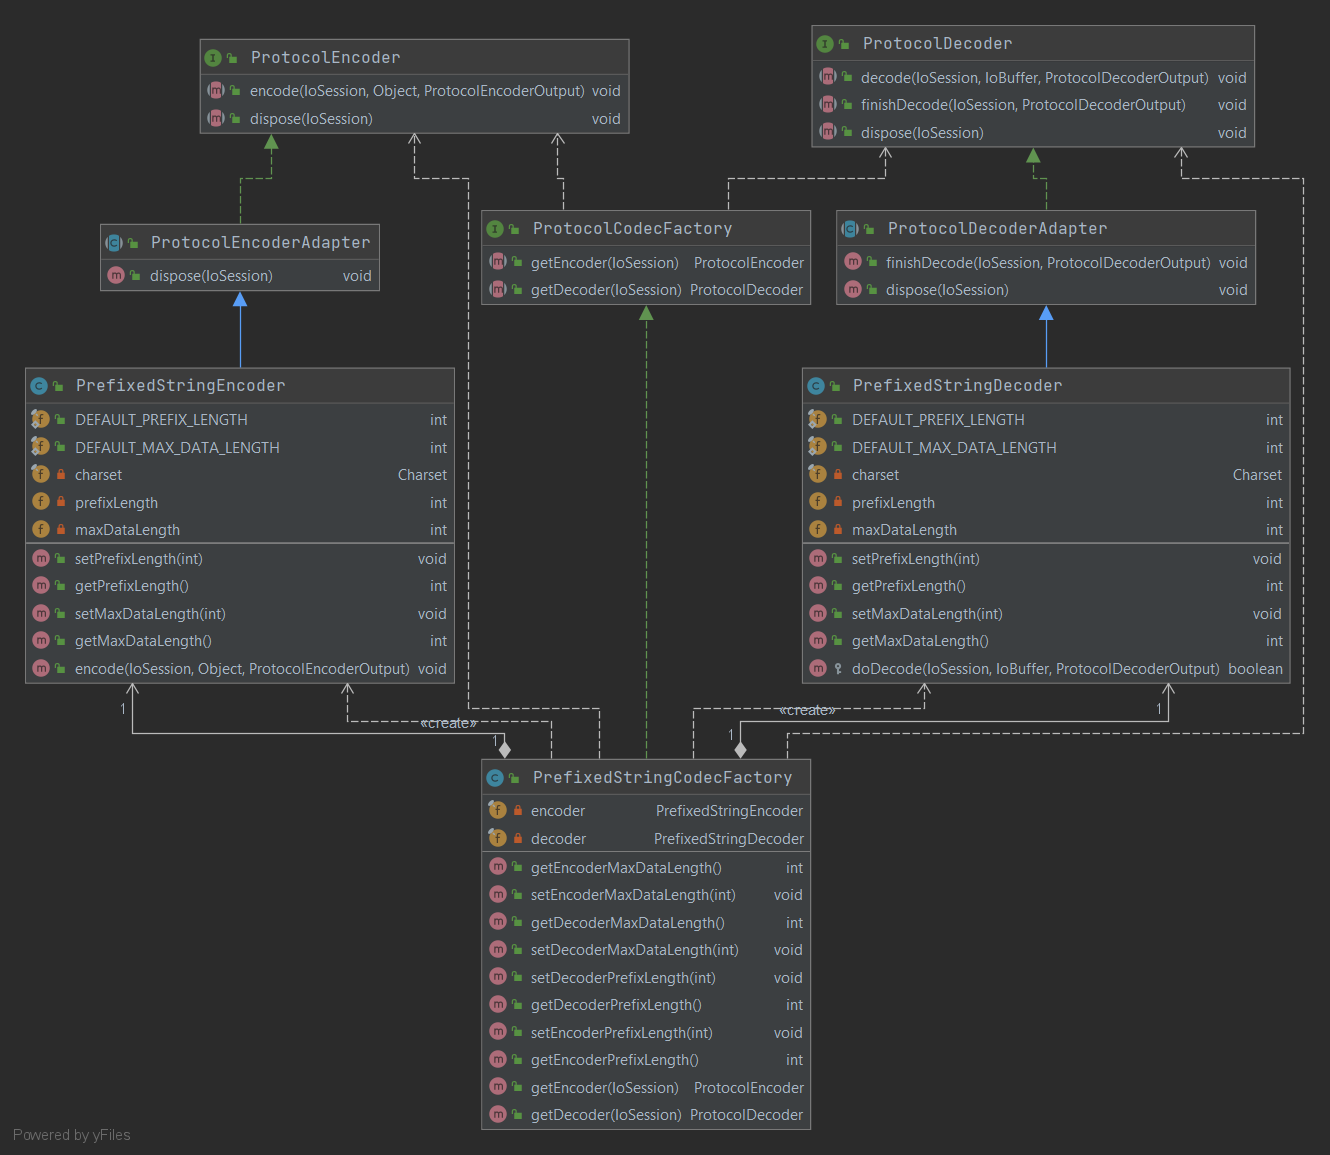
\includegraphics[width = \textwidth]{images/class_diagrams/adapter_facade_pattern.png}
    \caption{Class diagram for the implementation of the Facade and Adapter patterns within the scope of the prefix codec filter.}
    \label{fig:cd_facade}
\end{figure}

\subsubsection{Current patterns: Factory pattern}
The above section presented an instance where the Factory pattern was incorrectly recovered as the Adapter pattern; we, thus, present 2 distinct instances of the Factory pattern where the pattern is correctly represented in the code base.\\\\
\textsc{Pattern definition}: The \textsc{Factory} pattern falls into the category of creational patterns and is one of the most used pattern in OO languages. This pattern provides an interface for creating objects in a superclass, while still allowing for the subclasses to alter the type of objects to be created. The creation logic is not exposed, the newly created objects can be referred to via the said interface \cite{factory}\cite{factory1}.\\\\
\textsc{Pattern implementation information from PINOT}
\begin{itemize}
    \item \textsc{Factory instance 1, recovered at intro commit \#832}
        \begin{itemize}
            \item \textsc{Factory Method Class}: \texttt{StateContextFactory}
            \item \textsc{Factory Method Result Base}: \texttt{StateContext}
            \item \textsc{Factory Method Implementation}: \texttt{DefaultStateContextFactory}
            \item \textsc{Factory Method Results}: \texttt{DefaultStateContext}
            \item \textsc{Factory Method}: \texttt{create}
        \end{itemize}
    \item \textsc{Factory instance 2, recovered at intro commit \#1522}
          \begin{itemize}
            \item \textsc{Factory Method Class}: \texttt{ByteArrayFactory}
            \item \textsc{Factory Method Result Base}: \texttt{ByteArray}
            \item \textsc{Factory Method Implementation}: \texttt{SimpleByteArrayFactory}
            \item \textsc{Factory Method Results}: \texttt{BufferByteArray}
            \item \textsc{Factory Method}: \texttt{create}
        \end{itemize}
\end{itemize}
\textsc{Implementations \& class diagrams}: The implementations of the Factory instances are presented in figures \ref{fig:factory1}, \ref{fig:factory2}. The specific factories (i.e. \texttt{DefaultStateContextFactory} and \texttt{SimpleByteArrayFactory}) implement the main Factory interface (i.e. \texttt{StateContextFactory} and \texttt{ByteArrayFactory}) and encapsulate the creation of specific objects, in this case \texttt{DefaultStateContext} and \texttt{BufferByteArray}, which are implementations of a superclass interface, \texttt{StateContext} and \texttt{ByteArray}, respectively. \\\\
\textsc{Issue tracking \& motivation}: The objects that are being created in both cases are meant to be used unaltered in order to ensure that the desired functionality of MINA. In the \texttt{byteaccess} context, the client should not be involved with the creation of the \texttt{BufferByteArray} objects since it cannot accept alterations: the \texttt{BufferByteArray} is part of the MINA specific low level API which uses custom byte buffers. The commit message corresponding the intro commit also indicates that pattern instance was impacted by the addition of a new feature (i.e. \textit{"Adding in the Composite IoBuffer code."}). Same situation goes for the \texttt{mina-statemachine} context: the \texttt{DefaultStateContext} object represents the default implementation of a \texttt{StateContext} which implies that it needs to inherit all the required aspects (i.e. stores the current state and all client specific information since all clients use the same \texttt{StateMachine} which is a Singleton) for the successful implementation of the state machine (see section \ref{sec:analysis_components}). Unlike the previous pattern discussed up until this point, the Factory pattern is well discussed between the developers of MINA. It also appears in relation with the 2 instances we discuss here. For the Factory pattern, the developers seem to be aware of the correct implementation of this pattern, as well as of its usage compatibility in various areas of the code base. This remark is also supported by the coherent naming of the factory files. The Factory pattern is most of the times mentioned in relation with codecs, however PINOT does not recover any current Factory instance within the \texttt{mina-filter} scope. An example of a mis-identification of the Factory pattern is mentioned in section \ref{sec:current_facade_adapter}.\\\\
\textsc{Impact on architecture}: The Factory instances presented do not have a significant impact on the overall architecture, however, the approach of using the Factory method for creational purposes spreads over multiple components in the current version of the code base (i.e. \texttt{mina-statemachine}, \texttt{mina-integration}, \texttt{mina-core-transport}, \texttt{mina-core-util}, \texttt{mina-core-IOFilterTypes}). From investigating the code and the developers discussions, we inferred that the Factory pattern could possibly have more instances in the code base than currently identified by PINOT.\\\\
\textsc{Preliminary conclusions}: The popularity of the Factory pattern is reflected in the frequency of its occurrence in the code base, as well as in the discussions between the developers. The development community is clearly aware of the existence and utility of this design pattern; the mailing list presents significant discussions about the implementation of this pattern. This is striking, since for the rest of the patterns we analysed the developers seem to have little or no understanding of the patterns as being part of the code base. This shows that the Factory method is, indeed, one of the most popular design patterns. \\\\
\textsc{Similar pattern instances}: The Factory pattern is recovered following a similar structure as presented before within the scope of \texttt{mina-integration-beans}. We present these pattern instances as well to analyse the reason behind their introduction. The Factory pattern is identified 5 times for 2 different intro commits: 
\begin{itemize}
    \item Intro commit \#1199:
        \begin{itemize}
            \item \textsc{Factory pattern instances}: the \texttt{factoryMethodClass} is \texttt{AbstractPropertyEditor} with 3 \texttt{factoryMethodImplementation}s: \texttt{URIEditor}, \texttt{URLEditor}, \texttt{FileEditor}.
            \item \textsc{Commit message}: the commit message suggests that the patterns instances have been introduced following the extension of the MINA integration, therefore due to the introduction of new functionality (i.e. \textit{"* Revamped JMX integration to make it work better with more POJO
    * Added more PropertyEditors to support JMX integration
    * Added PropertyTypeConverter to OGNL integration module"}).
        \end{itemize}
    \item Intro commit \#1851:
        \begin{itemize}
            \item \textsc{Factory pattern instances}: the \texttt{factoryMethodClass} is \texttt{AbstractPropertyEditor} with 2 \texttt{factoryMethodImplementation}s: \texttt{InetSocketAddressEditor}, \texttt{VmPipeAddressEditor}.
            \textsc{Commit message}: Commit \#1851 marks the module refactoring. 
        \end{itemize}
\end{itemize}

\textsc{Total number of pattern instances analysed:} 7 pattern instances with intro commit numbers \#832, \#1522, \#1199, \#1851.

\begin{figure}[H]
    \centering
    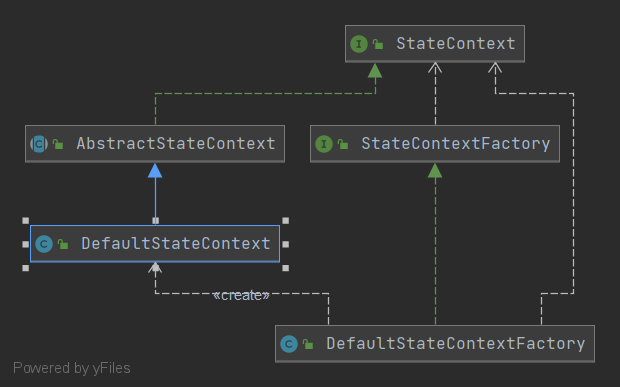
\includegraphics[width = 0.7 \textwidth]{images/class_diagrams/factory1.png}
    \caption{Class diagram of the Factory pattern instance recovered from \texttt{mina-statemachine}}
    \label{fig:factory1}
\end{figure}

\begin{figure}[H]
    \centering
    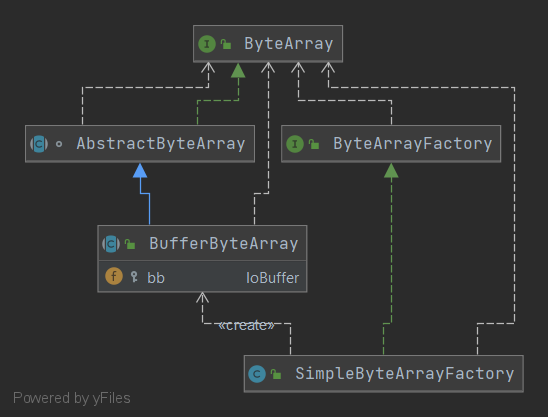
\includegraphics[width = 0.6 \textwidth]{images/class_diagrams/factory2.png}
    \caption{Class diagram of the Factory pattern instance recovered from \texttt{byteaccess}}
    \label{fig:factory2}
\end{figure}

\subsubsection{Removed patterns: Strategy pattern}
This section discusses the Strategy pattern within the scope of the \texttt{IoService} class. PINOT has recovered multiple instances of this pattern implemented in the \texttt{IoService} class throughout the analysed commit history; a variant of this pattern still exists in the current version of MINA. This shows that, despite its variations (which resulted in multiple pattern instances recovered), the Strategy pattern implemented in the \texttt{IoService} class can be considered a `fundamental' pattern since it persisted until the current version of MINA. This also holds for other instances of the Strategy pattern found in similar scopes (e.g. \texttt{IoSession}). With the analysis of this Strategy pattern we aim at comparing its initial and final implementations, as well as investigating for revelatory clues of the changes that occurred in between.\\\\
\textsc{Pattern definition}: \textsc{Strategy} is a behavioural design pattern which allows for different class behaviours, which can be chosen at run time. Multiple strategy implementations are defined which extend the main strategy interface; a context object represents the context in which the strategy should be applied. Based on the chosen strategy implementation, the behaviour of the context object is subject to change \cite{strategy}\cite{strategy1}.\\\\
\textsc{Pattern implementation information from PINOT}:
\begin{itemize}
    \item \textsc{Initial instance}:
        \begin{itemize}
            \item \textsc{Strategy file}: \texttt{IoService}
            \item \textsc{Implementations}: 17 strategy implementations (see figure \ref{fig:strategy_removed})
            \item \textsc{Contexts}: \texttt{VmPipeSessionImpl}, \texttt{DatagramSessionImpl}, \texttt{SocketSessionImpl}
            \item \textsc{Delegator}: \texttt{IoService manager} in each of the contexts. 
        \end{itemize}
    \item \textsc{Current instance}:
        \begin{itemize}
            \item \textsc{Strategy file}: \texttt{IoService}
            \item \textsc{Implementations}: 7 strategy implementations (see figure \ref{fig:strategy_current})
            \item \textsc{Contexts}: \texttt{DefaultSocketSessionConfig}, \texttt{IoServiceStatistics}
            \item \textsc{Delegator}: \texttt{IoService parent}, \texttt{IoService service} 
        \end{itemize}
\end{itemize}
\textsc{Implementation \& class diagram}: The implementations of the strategy are captured by figures \ref{fig:strategy_removed} and \ref{fig:strategy_current}. The \texttt{IoService} is the backbone of any MINA based application (see section \ref{sec:analysis_components}); it needs to `adapt' based on the type of network communication (i.e. TCP, UDP or in VM communication) and the participant to the communication (i.e. either a server, acceptor, or a client, connector). This idea is being concretized by the concept behind the Strategy pattern, where the \texttt{IoService} is the base strategy and the strategy implementations correspond with the above mentioned `adaptations'. The strategies can be accessed through a \texttt{delegator}, a basic \texttt{IoService} object which expose the different implementations. In the initial Strategy pattern (see figure \ref{fig:strategy_removed}) a larger variety of implementations is present; in the latest version (see figure \ref{fig:strategy_current}), the number of strategy implementations has been reduced to a small number of essential interfaces which can further facilitate the user implementation of more specific strategies for their applications (e.g. \texttt{AbstractIoService} which stands as a base implementation for \texttt{IoService}); also, the in VM communication is not explicitly treated as a strategy. The contexts also differ between the initial and final version: the initial version employed the Strategy pattern in the context of defining base session implementations for each of the communication types, while in the final version, only one default or base implementation is presented (the level of generalization here is higher than in the initial version). Moreover, the final version introduces the \texttt{IoServiceStatistics} which corresponds to a more recent feature which provides statistics about number of connections, idle times etc.\\\\
\textsc{Issue tracking \&  motivation}: The motivation of introducing this pattern has been touched upon within the implementation discussion above. What is interesting to us, is the motivation behind the changes that occurred to this pattern throughout the commit history; we identify the following motivations based on the commit messages related to this pattern, an overview of the data identified to support these motivations is presented in Appendix \ref{sec:strategy_motivation}:
\begin{itemize}
    \item Resolving issues (mostly, JIRA listed) by improving the pattern or removing elements from it.
    \item Updates or improvements to the code to fit the growth of the project as a whole. For example:
    \item Renamings/refactorings or updates needed for integration or maintenance purposes. For example:
\end{itemize}
We traced the changes and motivations over 42 Strategy patterns instances analysed within the \texttt{IOService} scope; the 42 instances span a timeline from commit \#41 to commit \#2545, we observe that the removal of a pattern instance is immediately (or very shortly) followed by the patterns re-introduction (also see figure \ref{fig:strategy_timeline}). Despite the alteration, the concept entailed by the Strategy pattern persisted within this scope, which means that the pattern was a good fit for the problem intended to solve. Discussion between developers regarding the implementation of this pattern is minimal, no concrete indicator towards the fact that they correlate having modeled multiple, behaviour changing variants of \texttt{IoService} to the Strategy pattern.

\textsc{Impact on architecture}: As it can be seen from figures \ref{fig:strategy_current} and \ref{fig:strategy_removed}, the number of classes required for the implementation of this pattern has reduced significantly from the introduction of the first instance. The current architecture reflects an emphasis on generalization and higher levels of abstraction. This is an indicator of how the project has matured over its development.

\textsc{Preliminary conclusions}: The chosen Strategy pattern instance seems to fit the context in which it has been introduced. Similar Strategy pattern approaches have also been taken for components that require the same `adaptations' as the \texttt{IoService} one. However, it is difficult to establish if the introduction of the pattern has been explicitly debated by the developers: from the mailing lists and JIRA tickets, there are little to no explicit mentions of this pattern. It might be the case that the developer community is not fully or actively aware of the existence of this pattern or that the choice made towards this implementation (which coincides with the implementation of a Strategy pattern) was not necessarily pursued to implement said pattern.  
\begin{landscape}
    \begin{figure}
    \centering
    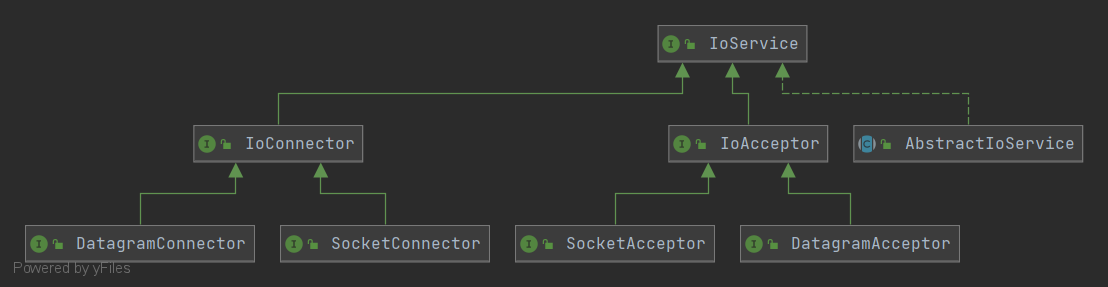
\includegraphics[width = \textwidth ]{images/class_diagrams/strategy_current.png}
    \caption{Class diagram of the the current Strategy pattern instance in \texttt{IoService}, capturing the strategy possible implementations; the context files are not shown in this diagram.}
    \label{fig:strategy_current}
\end{figure}
    \begin{figure}
        \centering
        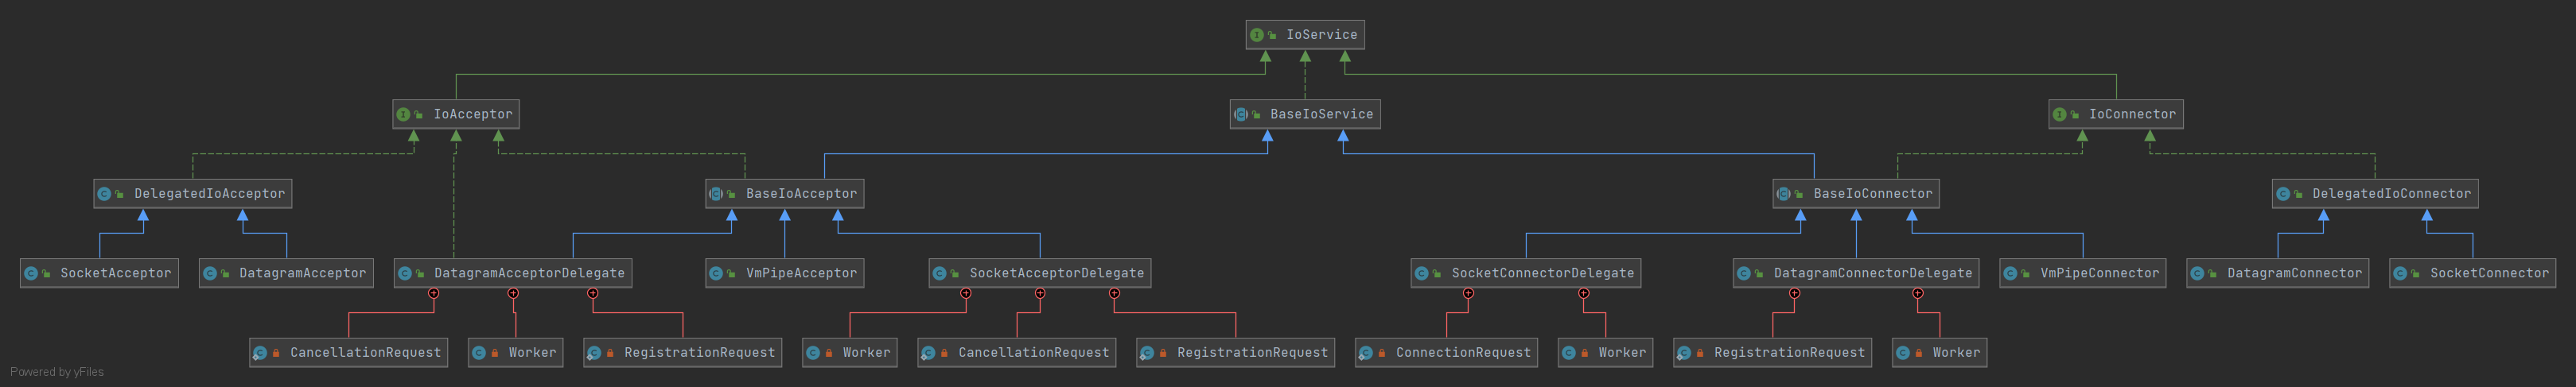
\includegraphics[scale = 0.2 ]{images/class_diagrams/strategy_removed.png}
        \caption{Class diagram of the initial (now removed) Strategy pattern instance in \texttt{IoService}, capturing the strategy possible implementations; the context files are not shown in this diagram.}
        \label{fig:strategy_removed}
    \end{figure}
\end{landscape}

\subsection{Removed patterns: Singleton, Chain of Responsibility, Template, Observer}
According to our quantitative analysis the Singleton, CoR (Chain of Responsibility), Template and Observer pattern types have been permanently removed from the code base. We will look into the motivation behind the permanent removal:
\begin{itemize}
    \item \textsc{Singleton}: the Singleton pattern was recovered for 6 instances in the context of monitoring the idle status of sessions, VM pipe connections and life cycle of IO filters. Out of the 6 instances none remained because the developers took a different approach to idle checking: the classes that were implemented as a singleton have been completely removed from the code base, the only class remaining is \texttt{IoSessioChecker} which is not a singleton any longer.
    \item \textsc{CoR}: the CoR pattern has been incorrectly recovered by PINOT for \texttt{CompositeByteArray} class which is an example of the Composite pattern.
    \item \textsc{Template}: the Template pattern has been identified for classes that presented a base implementation of an interface, for example \texttt{BaseIOAcceptor} which implemented the  \texttt{IOAcceptor} interface. Most of the classes that implemented the Template pattern were removed from the code base during code clean ups; moreover, the remaining \texttt{BaseInterface} were renamed to \texttt{AbstractInterface}, however PINOT does not recognize them as Templates any longer.
    \item \textsc{Observer}: The Observer pattern was recovered in the following contexts:
    \begin{itemize}
        \item \texttt{ThreadPoolFilter}: this filter has been removed
        \item \texttt{LeaderFollowerThreadPool}: this threading pattern is no longer supported in the current code version
        \item \texttt{StatCollector}: for statistics, the \texttt{IOServiceStatistics} has been implemented and is currently present in the final code version
        \item \texttt{IoServiceListenerSupport}: the \texttt{IoServiceListenerSupport} is no longer an instance of the Observer pattern since it is implemented in such a way that it does not have a specific subject
        \item \texttt{DefaultIoFuture}: currently it is implemented with threading, therefore a different approach has been taken
        \item \texttt{CompositeByteArray}: currently this class implements the Composite pattern
        \item \texttt{DecodingStateProtocolDecoder}: removed permanently from the \texttt{mina-statemachine} scope of the project; the functionality is no longer required
    \end{itemize}
    
\end{itemize}

\subsection{Mailing list analysis}
\label{sec:malilinglist_analysis}
We further analyse the mailing list for all types of patterns discovered by PINOT. The following list shows which of the identified patterns are being discussed among the developers via the MINA mailing lists:
\begin{itemize}
    \item Patterns which appear in mailing list discussion: 
        \begin{itemize}
            \item Visitor
            \item Observer
            \item Proxy (discussed, but not clear if they aware that it represents a design pattern)
            \item Singleton \& Multiton
            \item Decorator
            \item Composite
            \item Chain of Responsibility (CoR)
            \item Factory
        \end{itemize}
    \item Patterns which are not explicitly mentioned in mailing list discussions:
        \begin{itemize}
            \item Mediator
            \item Bridge
            \item Flyweight
            \item Template
            \item Strategy
            \item Facade (very limited and unrelated discussion)
            \item Adapter (very limited discussion)
        \end{itemize}
\end{itemize}
We observe from the list above that the design patterns that are being discussed are fairly common; they are mentioned in very specific contexts, for example, the CoR pattern is considered for the implementation of filter chaining; the Visitor pattern is only mentioned in the context of the out-of-the-box demuxing handler implementation; the Composite pattern is only related to the \texttt{ByteArray} interface and byte array support. From these discussions, it becomes apparent that the developers are experienced and know how to identify situations in which using design patterns is suitable. However, there are only a couple of instances (for example, the CoR pattern in relation with the filter chain) when patterns are discussed when planing is done for a future component implementation. Most times, pattern discussion coincides to discussion threads that deal with solving some sort of issue. This enforces our earlier assumption about patterns being introduced \textit{a posteriori}.\\\\
At the same time, the lack of discussion about some of the patterns recovered hints towards the fact that the developers might not be aware of the patterns' implementation in the code base. For patterns such as Strategy and Mediator, it might be the case that they are implicitly introduced since they can be seen as following from best coding practices. An intriguing example is the case of the Adapter pattern: the developers discuss the \textit{lack} of this pattern in the code base, despite many class names containing the "adapter" keyword. \\\\
Apart from GoF design patterns, the developers also seem to briefly discuss enterprise integration patterns (EAP), as well as threading models (e.g. Leader-Follower).